\documentclass[smaller,notes=hide]{beamer}
\usepackage[english]{babel}
\usepackage{multimedia}
\usepackage{bm}
%\usepackage{mathrsfs}
\usepackage{mathtools}
\usepackage{amsmath}
\usepackage{pgf,textcomp}
\usepackage{pict2e} 
%\usepackage[utf8]{inputen}
%\usefonttheme[onlymath]{serif}

\usepackage[latin1]{inputenc}

\usepackage{times}
\usepackage{helvet}

\usepackage{hyphenat}
\usepackage{caption}
\captionsetup[figure]{labelfont = bf, name = Fig., format = plain, margin = 1pt}

%Bibliography
%\usepackage{bibgerm}
\usepackage[backend=biber, style = phys,maxnames=4,clearlang=true,doi=false]{biblatex}
\usepackage{csquotes}
\setlength{\tabcolsep}{18pt}
%\DeclareRedundantLanguages{english,german,french,en,de}{english,german,french,en,de}
\addbibresource{talk.bib}

\defbibfilter{papers}{
	type=article or
	type=inproceedings or
	type=incollection
} 



\graphicspath{{../plots/}}

\definecolor{myblue}{rgb}{0.1,0.4,0.7}
\definecolor{gray}{rgb}{0.5,0.5,0.5}
\definecolor{lightyellow}{rgb}{0.98,0.95,0.6}
%\definecolor{myblue}{rgb}{0.1,0.4,0.7}
\definecolor{myorange}{rgb}{0.8,0.4,0.0}
\definecolor{mypink}{rgb}{0.7,0.2,0.5}
\definecolor{lightblue}{rgb}{0.81,0.91,1.0}
\definecolor{mygreen}{rgb}{0.05,0.5,0.08}
\definecolor{myred}{rgb}{0.7,0.1,0.2}
\definecolor{darkblue}{rgb}{0.1,0.1,0.6}

\newcommand{\todo}[1]{\textcolor{red}{#1}}

\mode<presentation>
{
  \usetheme{Madrid}
  %\usetheme{Dresden}
  %\usecolortheme{seahorse}
  %\usecolortheme{orchid}
  \usecolortheme[named=myblue]{structure}
  %\useoutertheme{infolines}
  \useinnertheme{default}
  % or ...

  \setbeamercovered{transparent}
  \setbeamertemplate{navigation symbols}{}
}

\setlength{\fboxrule}{1pt}

\newcommand{\withbox}[2]{\setlength{\fboxsep}{0pt}\begin{center}\fcolorbox{darkblue}{lightblue}{\parbox{#1}{\begin{center}{#2}\end{center}}}\end{center}}
\newcommand{\strong}[1]{\textcolor{myred}{\bf #1}}
\newcommand{\question}[1]{\textcolor{mygreen}{\bf{#1}}}
\newcommand{\mymath}[1]{\textcolor{darkblue}{#1}}
\newcommand{\subt}[1]{\textcolor{darkblue}{\underline{\bf #1}}\\ \vskip0.3cm}
\newcommand\at[2]{\left.#1\right|_{#2}}
\newlength{\wideitemsep}
\setlength{\wideitemsep}{\itemsep}
\addtolength{\wideitemsep}{2pt}
\let\olditem\item
\renewcommand{\item}{\setlength{\itemsep}{\wideitemsep}\olditem}

\def\tril{\mbox{\begin{picture}(5,5)
\put(1,0){\line(1,0){5}}
\put(6,0){\line(-1,1){5}}
\put(1,0){\line(0,1){5}}
\end{picture}
}}


\newcommand{\triu}{\mathbin{\rotatebox[origin=c]{180}{$\tril$}}}

\title[Master Colloquium]{\large Nucleation and Crystallization of the
Metastable Hard Sphere Fluid}

\author[W. W\"ohler]{Wilkin W\"ohler}
\institute[]{Universit\"at Freiburg}
\date{14.5.2021}

%\beamerdefaultoverlayspecification{<+->}

\begin{document}

\begin{frame}[plain]
  \begin{center}
    \setlength{\fboxsep}{0pt}
      \begin{center}
        \fcolorbox{lightblue}{lightblue}{\parbox{10cm}{
          \begin{center}
            {\large Nucleation and Crystallization of the
Metastable Hard Sphere Fluid - Master Colloquium}
          \end{center}}
        }
      \end{center}
    \vfill
    {Wilkin W\"ohler,\\ Albert-Ludwigs-Universit\"at Freiburg}
    \vfill    
    {\small{\today}}
  \end{center}
\end{frame}

\begin{frame}
  \frametitle{Content}
  \begin{itemize}
    \item Introduction
    \begin{itemize}
      \item Metastable hard sphere fluid
      \item Memory effects in non-stationary processes
      \item Nucleation rate discrepancy
    \end{itemize}
    \item Simulation scheme and testing
    \item Cluster growth rate
    \item Nucleation rate
    \begin{itemize}
      \item Definition
      \item Estimation
      \item Comparison
    \end{itemize}
    \item Memory kernel shape analysis
  \end{itemize}
\end{frame}



\begin{frame}
\frametitle{The Hard Sphere Fluid}
\begin{columns}
\column{0.5 \linewidth}
\begin{itemize}
\item Simplest model of a fluid
\begin{equation*}
\label{eqn:hs_potential}
V(r_{ij})=%\infty \cdot \Theta(\sigma - r_{ij})
\begin{cases}
\infty \quad & r_{ij} \le \sigma \\
0 \quad & r_{ij} > \sigma
\end{cases}
\end{equation*}
\vspace{-0.10cm}
\item Experimentally and theoretically studied
\vspace{0.25cm}
\item Liquid-Solid phase transition
\begin{itemize}
\item $\eta_{RCP} \approx{64\%}$,  $\eta_{HCP} \approx{74\%}$ %\\
%\quad $\Rightarrow$ Entropy increase
\item Entropy increase
\end{itemize}
\end{itemize}

%Equations of state:\\
%Carnahan-Starling\cite{Carnahan1969}
%\begin{equation}
%\label{eqn:CS}
%Z=\frac{1+\eta+\eta^2-\eta^3}{(1-\eta)^3}
%\end{equation}

%Almarza \cite{Almarza2009}
%\begin{equation}
%\frac{p(v-v_0)}{k_B T} = 3 - 1.807846 y + 11.56350 y^2 + 141.6 y^3 - 2609.26 y^4 + 19328.09 y^5
%\end{equation}
\column{0.025 \linewidth}
\column{0.45 \linewidth}

\begin{figure}[h]
\centering
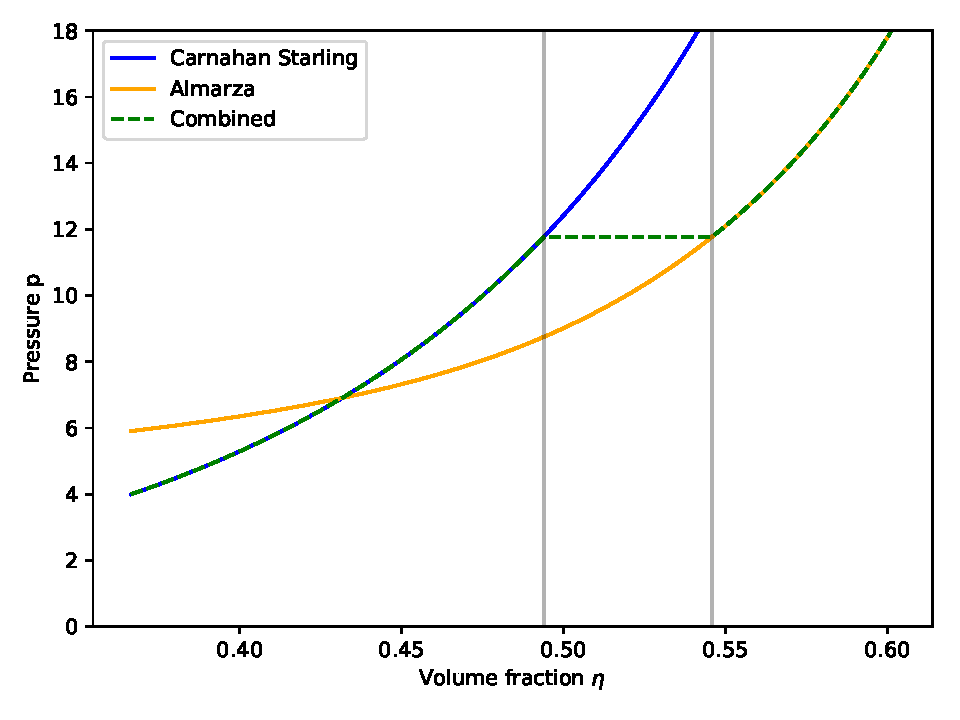
\includegraphics[width=1 \linewidth]{Hard_sphere_phase_diagram.pdf}
\caption[]{Carnahan-Starling\cite{Carnahan1969}, Almarza\cite{Almarza2009} and equilibrium equation of state}
\label{fig:hs_phase_diagram}
\end{figure}
\column{0.025 \linewidth}
\end{columns}
\end{frame}


% begin Choosing short or long crytallization part (LSCP)

\iffalse

\begin{frame}
\frametitle{Nucleation and Crystallization - \\ \hfill Phase Transitions}
\begin{itemize}
\item Technological and scientific importance
%\begin{itemize}
%\item Metallurgy, Atmosphere physics, ...
%\end{itemize}
%\vspace{0.5cm}
\item Commonly described by classical nucleation theory\\
\only<1>{$\quad \rightarrow$ qualitatively correct\\}
\only<1>{$\quad \rightarrow$ quantitatively not accurate}
\vspace{0.5cm}
\item<1> Other Approaches
\begin{itemize}
\item Modifying the free energy landscape
\item Markovian reaction coordinates
\item Memory effects
\end{itemize}
\end{itemize}
%\item Hard sphere nucleation rate discrepancy
\end{frame}

\fi

% inter Choosing short or long crytallization part (LSCP)

\iftrue

\begin{frame}
\frametitle{Nucleation and Crystallization - \\ \hfill Phase Transitions}
\begin{itemize}
\item Technological and scientific importance
%\begin{itemize}
%\item Metallurgy, Atmosphere physics, ...
%\end{itemize}
%\vspace{0.5cm}
\item Commonly described by classical nucleation theory\\
\only<0>{$\quad \rightarrow$ qualitatively correct\\}
\only<0>{$\quad \rightarrow$ quantitatively not accurate}
\vspace{0.5cm}
\item<0> Other Approaches
\begin{itemize}
\item Modifying the free energy landscape
\item Markovian reaction coordinates
\item Memory effects
\end{itemize}
\end{itemize}
%\item Hard sphere nucleation rate discrepancy
\end{frame}

\begin{frame}
\frametitle{Classical Nucleation Theory (CNT)}
\begin{columns}
\column{0.5 \linewidth}
\begin{itemize}
\item Spherical clusters
\item Coarse grained observable R
\item $\Delta F = 4 \pi R \gamma_{fs} - \frac{4 \pi}{3} R^3  \rho \,\Delta |\mu| $
\item<2> Markovian fluctuations
\item<2> Nucleation rate $\kappa  \propto \exp \left( -\frac{\Delta F}{k_B T} \right) $

\end{itemize}
\column{0.025 \linewidth}
\column{0.45 \linewidth}
  \centering
  \only<1>{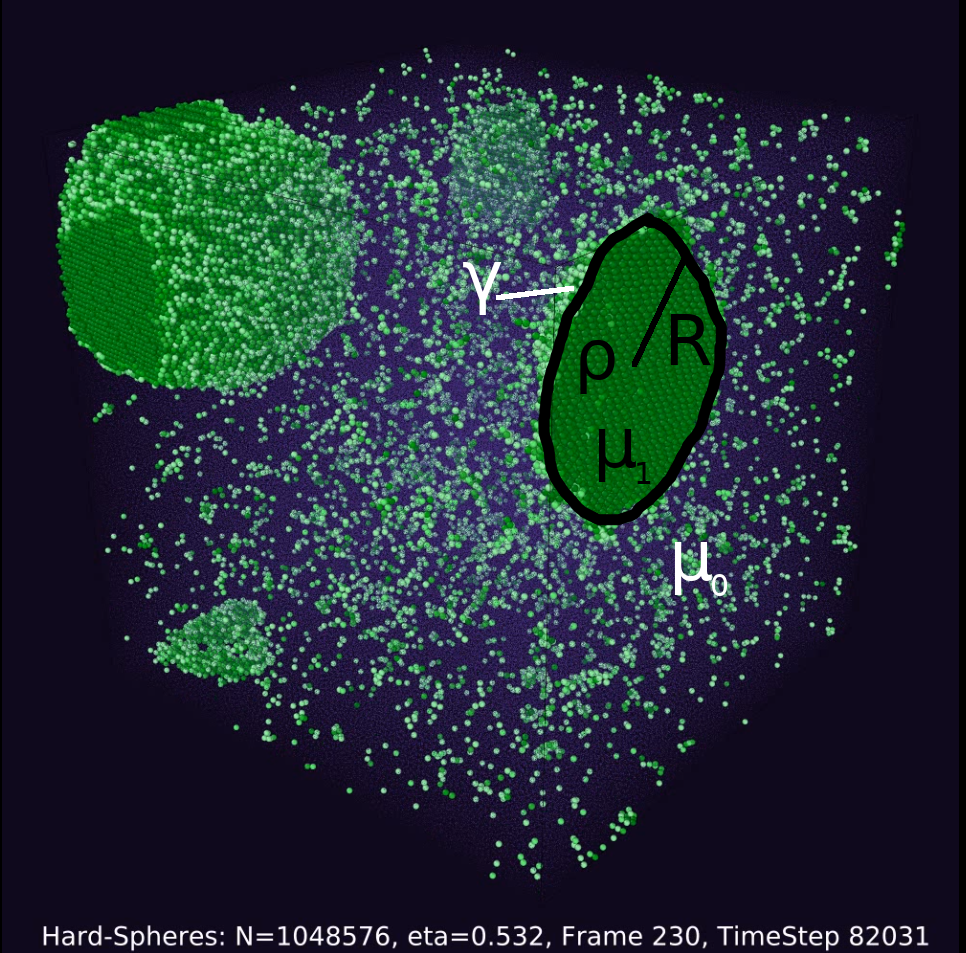
\includegraphics[width=1\linewidth]{animation_poster_532.png}}
  \only<2>{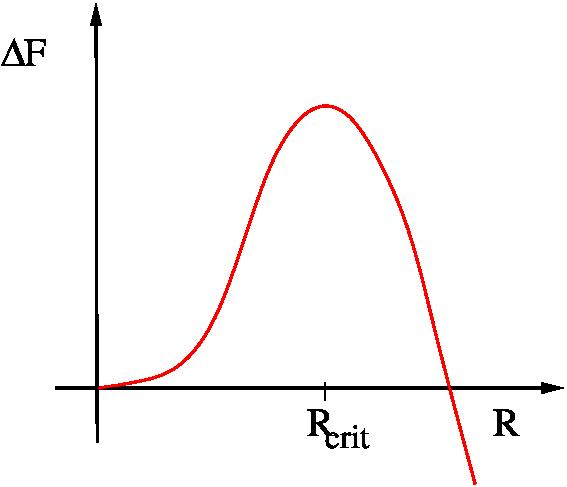
\includegraphics[width=1\linewidth]{CNTBarrier.jpg}}
\column{0.025 \linewidth}
\end{columns}
\end{frame}



\begin{frame}
\frametitle{Nucleation and Crystallization - \\ \hfill Phase Transitions}
\begin{itemize}
\item Technological and scientific importance
%\begin{itemize}
%\item Metallurgy, Atmosphere physics, ...
%\end{itemize}
%\vspace{0.5cm}
\item Commonly described by classical nucleation theory\\
\only<1>{$\quad \rightarrow$ qualitatively correct\\}
\only<1>{$\quad \rightarrow$ quantitatively not accurate}
\vspace{0.5cm}
\item Other Approaches
\begin{itemize}
\item Modifying the free energy landscape
\item Markovian reaction coordinates
\item Including memory effects
\end{itemize}
%\item Hard sphere nucleation rate discrepancy
\end{itemize}
\end{frame}

\fi
% end Choosing short or long crytallization part (LSCP)



\begin{frame}
\frametitle{Memory Effects Nucleation Processes}
Earlier work in the group:
\vspace{0.1cm}
\begin{itemize}
\item Memory effects observed in Lennard-Jones nucleation, Anja\cite{Kuhnbold2019}
\vspace{0.5cm}
\item Non-stationary generalized Langevin equation, Hugues\cite{MeyerThesis}
\begin{equation*}
\label{eqn:EOM_A}
  \frac{d A_{t}}{dt} = \omega (t) A_{t} + \int_{0}^{t} K(\tau, t) A_{\tau} d\tau + \eta_{0,t}
\end{equation*}
\item Non-Markovian kernel in the Lennard-Jones nucleation, Philipp P.\cite{ThesisPhilipp}
\end{itemize}
\vspace{0.5cm}
This work:
\vspace{0.1cm}
\begin{itemize}
\item Memory kernel of hard sphere nucleation process
\end{itemize}
\end{frame}






\begin{frame}
\frametitle{Nucleation Rate Discrepancy}
\begin{columns}
\column{0.5 \linewidth}
\begin{itemize}
\item Steeper decrease in simulations
%\end{itemize}
%\vspace{0.5cm}
\item Possible differences:
\begin{enumerate}
\item Hydrodynamics
\item Sedimentation
\item Polydispersity
\item Measurement geometry
\item ...
\end{enumerate}
\end{itemize}
\column{0.5 \linewidth}
\begin{figure}[h]
\centering
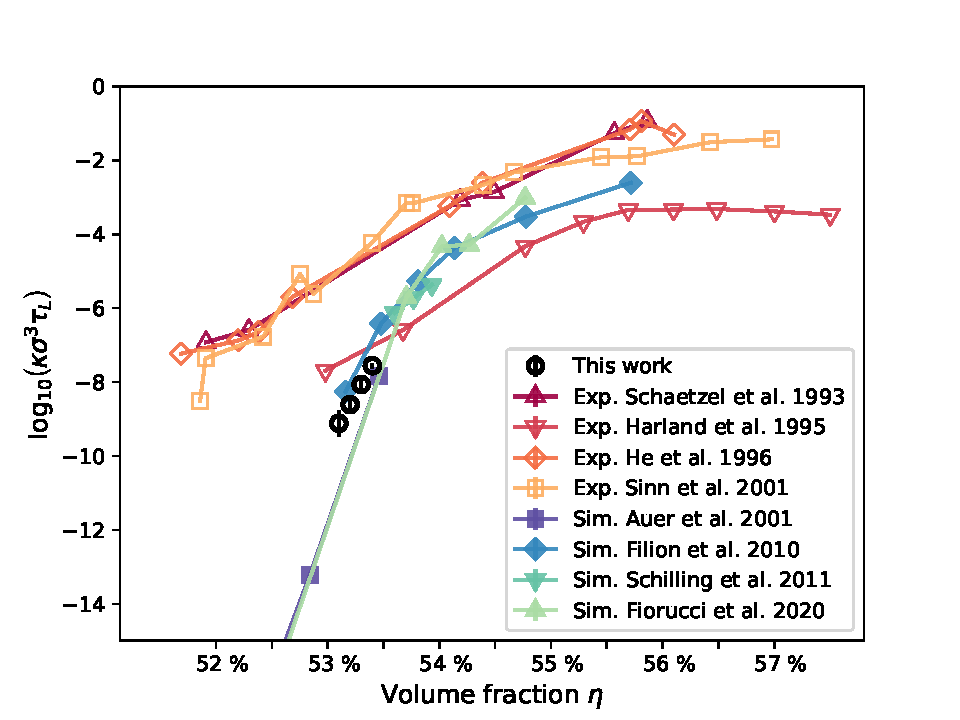
\includegraphics[width=1 \linewidth]{nucleation_comparison_v2.pdf}
\caption[]{Experimental and theoretical nucleation rates \cite{Harland1997,He1996,schaetzel1993,Sinn2001,Auer2001,Filion2010a,Fiorucci2020a,Schilling2011}}
\label{fig:nucleation_comparison}
\end{figure}
\end{columns}
%\begin{column}
%\end{column}
\end{frame}

\begin{frame}
\frametitle{Simulation Scheme and Testing}
\begin{columns} 

\column{0.5 \linewidth} 
Event driven molecular dynamics (EDMD)
\begin{itemize}
\item Discontinuous potential
\item Resolve dynamics
\item Based on analytical-
\begin{itemize}
\item ballistic trajectory
\item collision time
\item collision outcome
\end{itemize}
\vspace{0.25cm}
\item<2-> Validated dynamics by diffusion
\item<3> Cell system \\
\quad $\Rightarrow \mathcal{O}(N)$ calculation effort
\end{itemize}


\column{0.5 \linewidth} 

\only<2>{
\begin{figure}[h]
\centering
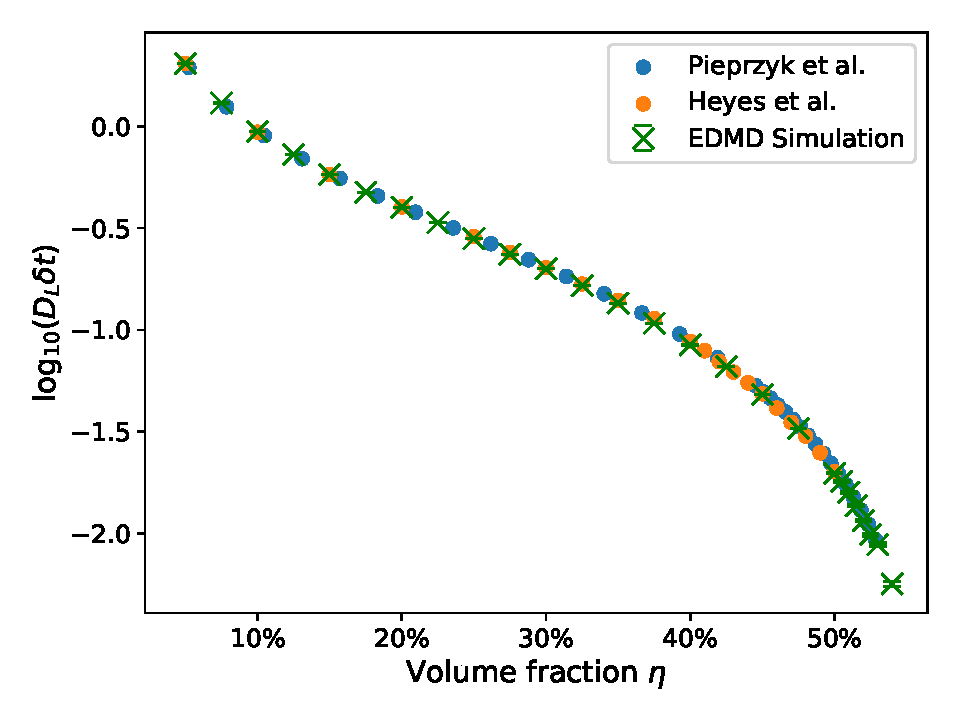
\includegraphics[width=1 \linewidth]{diffusion_probe.pdf}
\caption[]{Logarithmic plot of long time diffusion constant \cite{Pieprzyk2019, Heyes2007}}
\label{fig:diffusion_const}
\end{figure}
}

\only<3>{
\begin{figure}[h!]
\centering
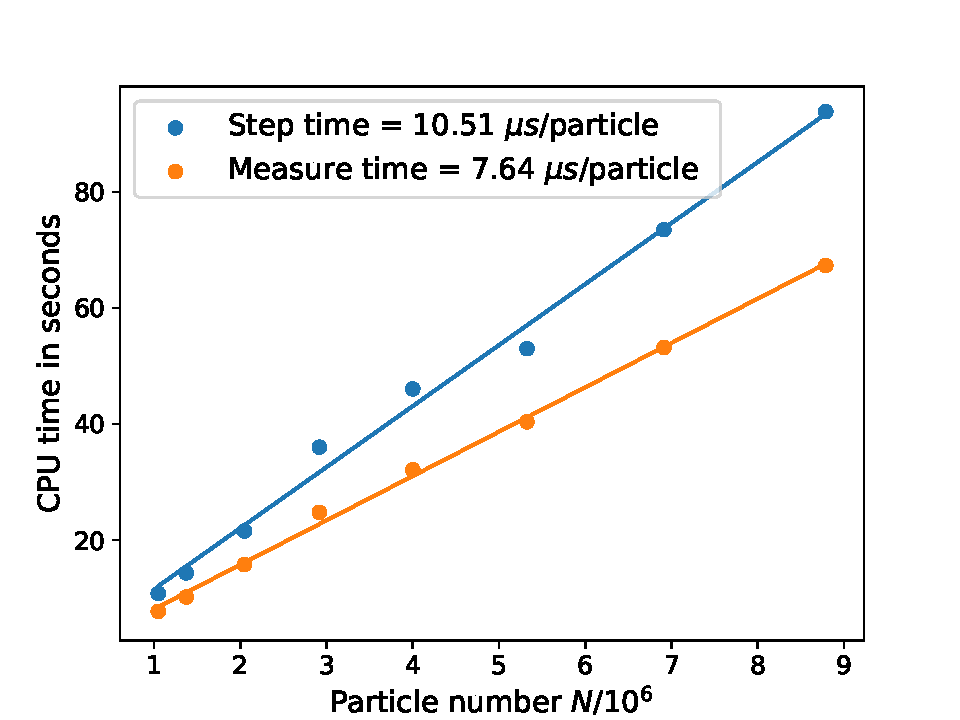
\includegraphics[width=1\linewidth]{Calculation_times_measurement.pdf}
\caption[]{CPU time per simulation step}
\label{fig:calc_time}
\end{figure}
}

\end{columns}
\end{frame}

\iffalse

\begin{frame}
\frametitle{EDMD I - Event Driven Molecular Dynamics}
\begin{itemize}
%\item Evolve each particle from collision to collision
\item Ballistic trajectories
\begin{equation*}
\vec{r}_i(t) = \vec{r}_i(t_0) + (t-t_0) \; \vec{v}_i(t_0)
\end{equation*}
\item Collision condition
\begin{align*}
f_{ij}(t)  &=  | \vec{r}_j(t) - \vec{r}_i(t) |^2 - \sigma^2\\
\Leftrightarrow \quad \Delta t &= \frac{ - rv - \sqrt{ (rv)^2  - vv (rr - \sigma^2 )} }{vv} \raisebox{-0.5cm}{ \makebox[0.1cm]{}} \\
\qquad \text{with } rr &\coloneqq |\vec{r}_{ij}(t_0)|^2  \text{, } vv \coloneqq |\vec{v}_{ij}(t_0)|^2   \text{ and }  rv \coloneqq \vec{r}_{ij}(t_0) \cdot \vec{v}_{ij}(t_0) \raisebox{-0.5cm}{ \makebox[0.1cm]{}} 
\end{align*}
%\item Evolve all particles to a certain time for measurements
%\vspace{0.0cm}
\item Collision outcome
\begin{align*}
%\label{eqn:collision_result}
\vec{v}_i^{\,'} = \vec{v}_i + \left( \frac{rv}{rr} \right) \vec{r}_{ij} 
\end{align*}
\end{itemize}
\vspace{0.25cm}
\hfill Based on Bannerman et al. 2014\cite{Bannerman2014}
\end{frame}

%\begin{frame}
%\frametitle{EDMD II - Collision Condition}
%
%\begin{align*}
%f_{ij}(t) & =  | \vec{r}_j(t) - \vec{r}_i(t) |^2 - \sigma^2
  %  & \; \; \, \vrule
  %\begin{aligned}[t]
  %  \quad \text{with} \quad \vec{r}_i(t) &= \vec{r}_i(t_0) + (t-t_0) \; \vec{v}_i(t_0) \, \text{,}\\
  %  \Delta t \coloneqq & \; t-t_0  \, \text{,} \\ 
  %  \vec{v}_{ij}(t) &\coloneqq  \vec{v}_j(t) - \vec{v}_i(t) \, \text{,}\\
  %  \vec{r}_{ij}(t) &\coloneqq  \vec{r}_j(t) - \vec{r}_i(t) \, \text{,}\\
  %  \Leftrightarrow \quad \vec{r}_{ij}(t) &= \vec{r}_{ij}(t_0) + \Delta t \; \vec{v}_{ij}(t_0)
  %\end{aligned}\\
%f(t)  & = ( \vec{r}_{ij}(t_0) +  \Delta t \;  \vec{v}_{ij}(t_0))^2 -\sigma^2 \\
%\label{eqn:overlap_f}
%f(t)  & = |\vec{r}_{ij}(t_0)|^2 + \Delta t ^2 \; |\vec{v}_{ij}(t_0)|^2 - 2 \Delta t \; \vec{r}_{ij}(t_0) \cdot \vec{v}_{ij}(t_0)  -\sigma^2
%\end{align*}  

%\begin{align*}
%\label{eqn:collision_prediction_pre}
%\Delta t &= \frac{ - rv - \sqrt{ (rv)^2  - vv (rr - \sigma^2 )} }{vv} \; \text{.}
%\end{align*}

%with  $rr \coloneqq |\vec{r}_{ij}(t_0)|^2  $, $vv \coloneqq |\vec{v}_{ij}(t_0)|^2  $ and  $ rv \coloneqq \vec{r}_{ij}(t_0) \cdot \vec{v}_{ij}(t_0) $


%\end{frame}

%\begin{frame}
%\frametitle{EDMD II - Collision Prediction}
%Event prediction algorithm by Bannerman et al. 2014\cite{Bannerman2014}:\\ \vspace{0.3cm}
%\begin{enumerate}
%\item $rv>0$, particles move away from each other  $\Rightarrow \Delta t = \infty$ \vspace{0.1cm}
%\item $rr<\sigma^2$, an overlap is present $\Rightarrow \Delta t = 0$\vspace{0.1cm}
%\item $(rv)^2  - vv (rr - \sigma^2 ) \leq 0 $, the particles miss each other $\Rightarrow \Delta t = \infty$\vspace{0.1cm}
%\item Otherwise, the particles collide $\Rightarrow \Delta t$\vspace{0.1cm}
%\end{enumerate}
%$\Rightarrow$ Resolves overlaps by direct collision
%\end{frame}

\begin{frame}
\frametitle{EDMD II - Evolution Cycle}
Initially:
\begin{enumerate}
\item Collisions and transfer prediction for each particle $\rightarrow$ PEL
\item First event of PEL to future event list (FEL)
\end{enumerate}
%\hrule 
\vspace{0.5cm}

Afterwards:
\begin{enumerate}
\item Draw first event from FEL
\item Execute event
\item Calculate new event(s)
\item Sort FEL
\item Restart at (1)
\end{enumerate}
\end{frame}



\begin{frame}
\frametitle{Simulation Characteristics and Testing}
\begin{columns}
\column{0.5 \linewidth}

\only<1>{
\begin{figure}[h!]
\centering
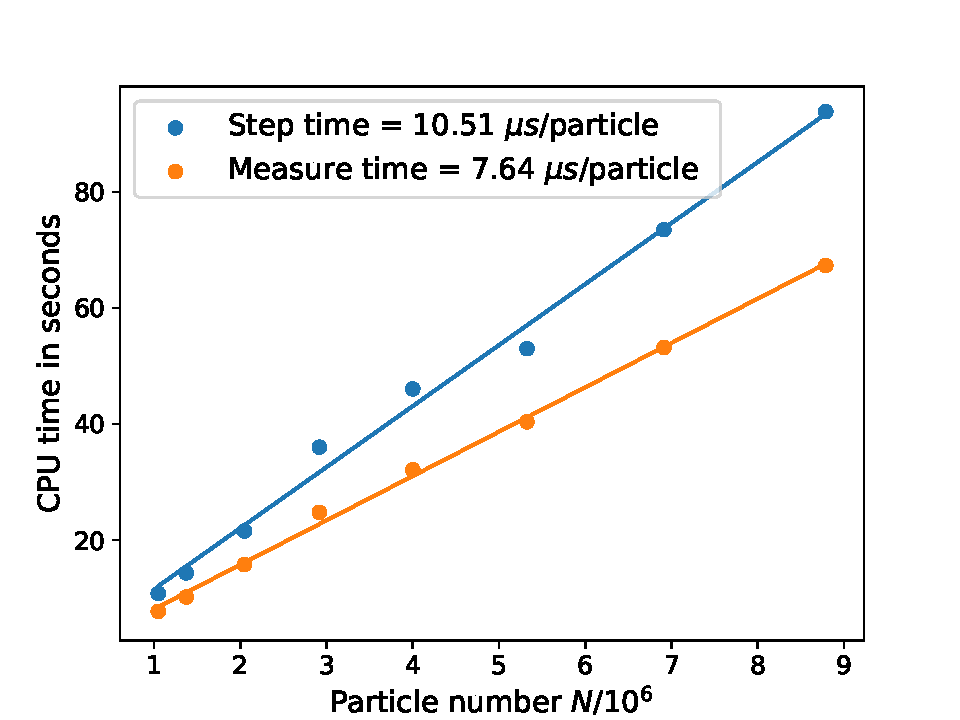
\includegraphics[width=0.94\linewidth]{Calculation_times_measurement.pdf}
\caption[]{CPU time per step}
\label{fig:calc_time}
\end{figure}
}

\only<2->{
\begin{itemize}
\item<2-> $\mathcal{O}(N)$ calculation effort
\item<2-> Chaotic behavior $\rightarrow$ rigorous saving
\item<3-> Validated diffusion
\item<4-> Validated RDF
\item<5-> Validating start parameters
\end{itemize}
}


\column{0.47 \linewidth}
\only<1>{
\begin{figure}[h!]
\centering
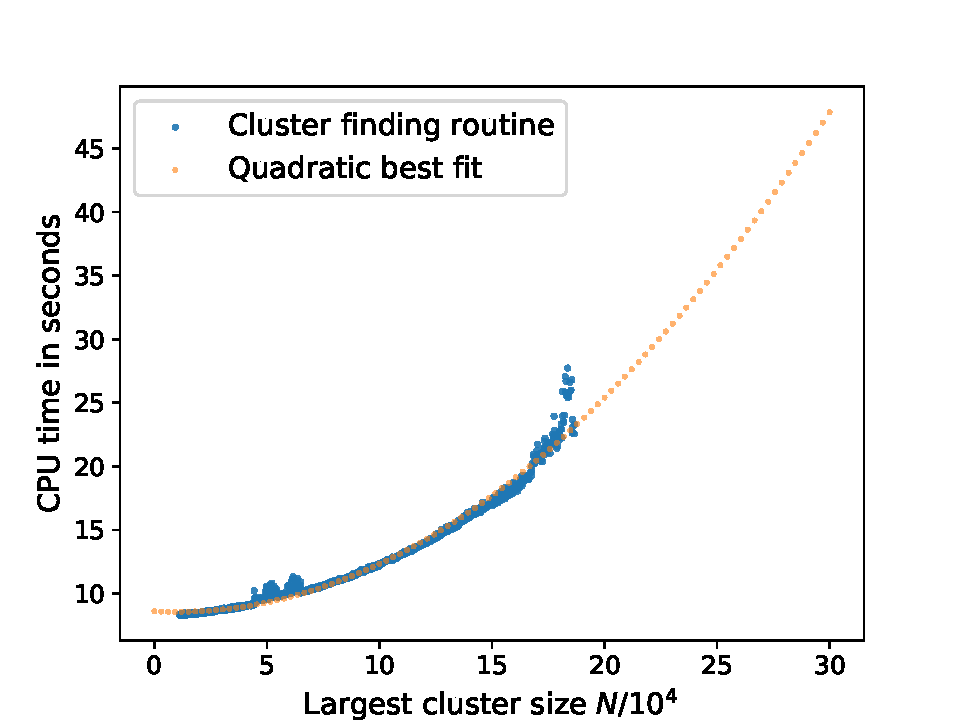
\includegraphics[width=1 \linewidth]{q6q6_calculation_time.pdf}
\caption[]{Cluster finding effort}
\label{fig:calc_q6q6}
\end{figure}
}

\only<2>{
\begin{figure}[h]
\centering
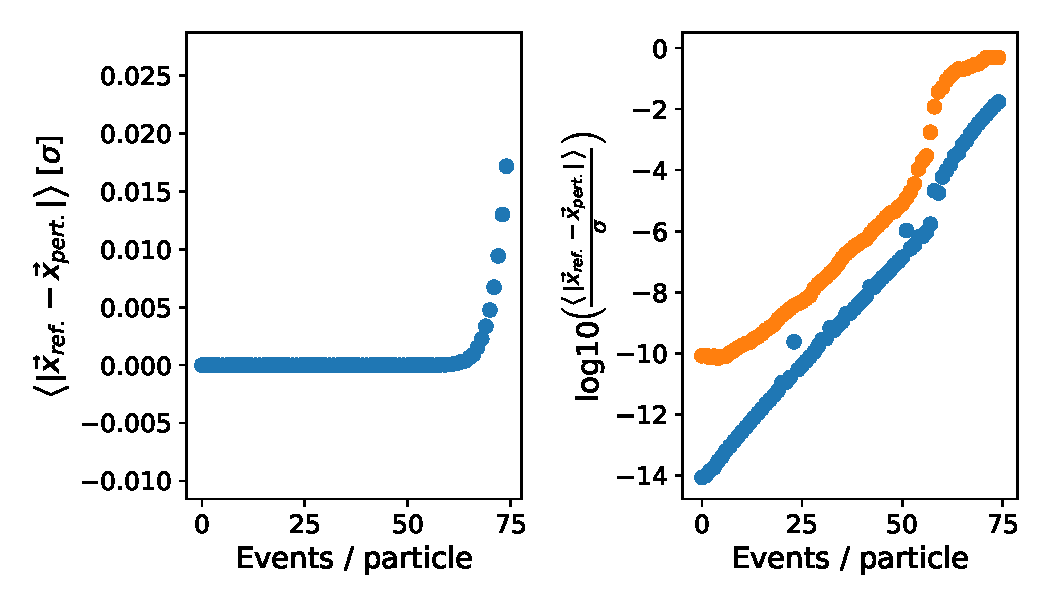
\includegraphics[width=1\linewidth]{perturbation.pdf}
\caption[]{Mean difference of positions in reference and perturbed simulation}
\label{fig:chaotic_behavior}
\end{figure}
}

\only<3>{
\begin{figure}[h]
\centering
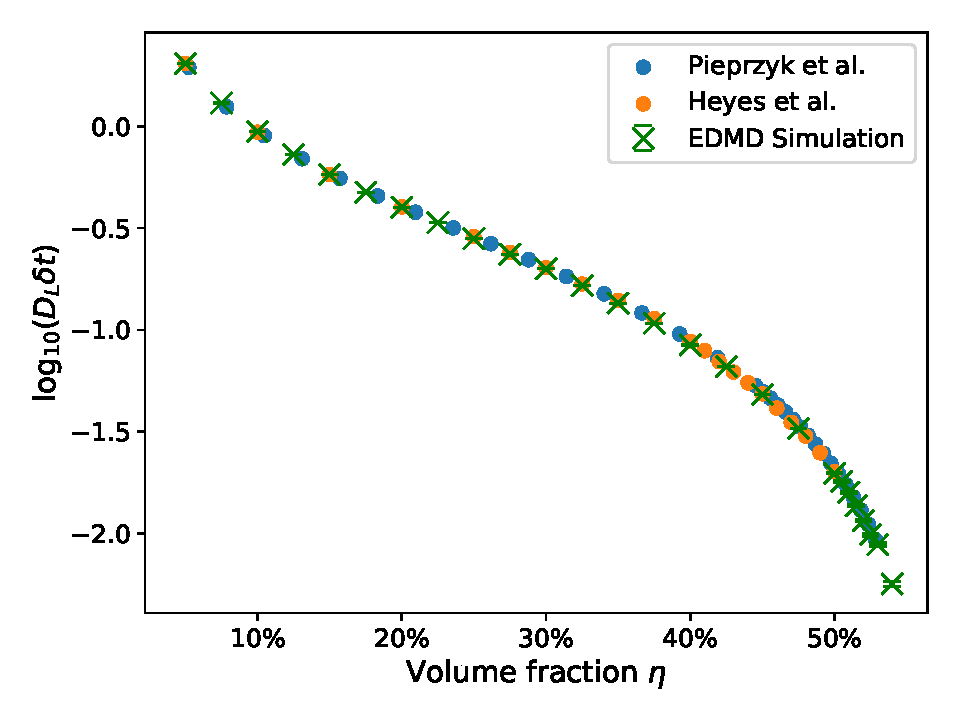
\includegraphics[width=1 \linewidth]{diffusion_probe.pdf}
\caption[]{Logarithmic plot of long time diffusion constant \cite{Pieprzyk2019, Heyes2007}}
\label{fig:diffusion_const}
\end{figure}
}

\only<4>{
\begin{figure}[h]
\centering
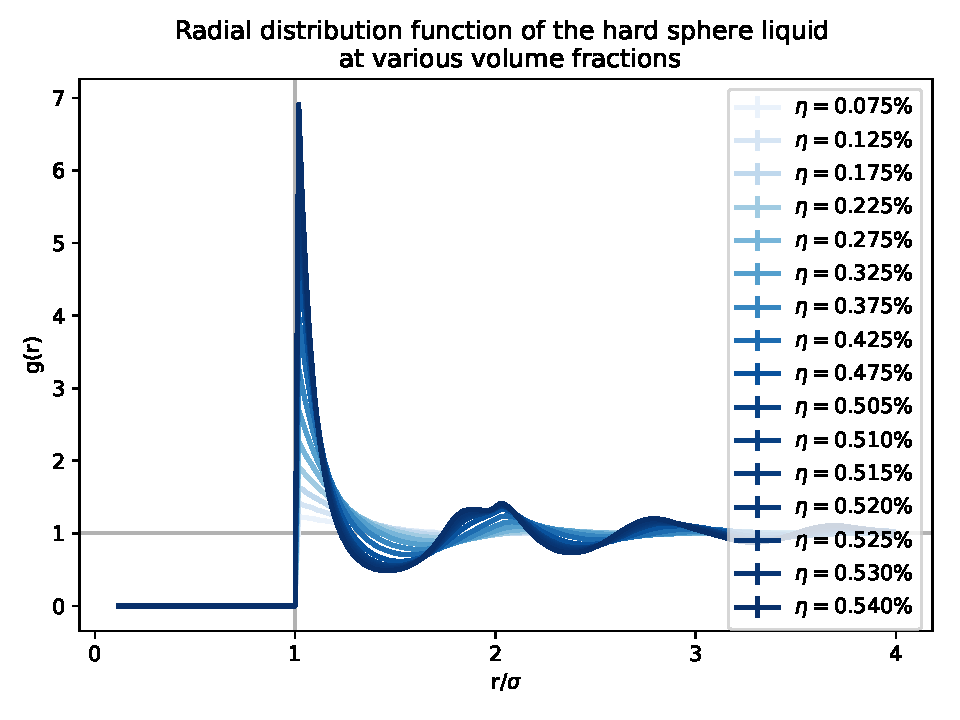
\includegraphics[width=1 \linewidth]{RDF.pdf}
\caption[Radial distribution functions at varying volume fractions]{Radial distribution functions (RDF)}
\label{fig:rdf_overview}
\end{figure}
}

\only<5>{
\begin{figure}[h!]
\centering
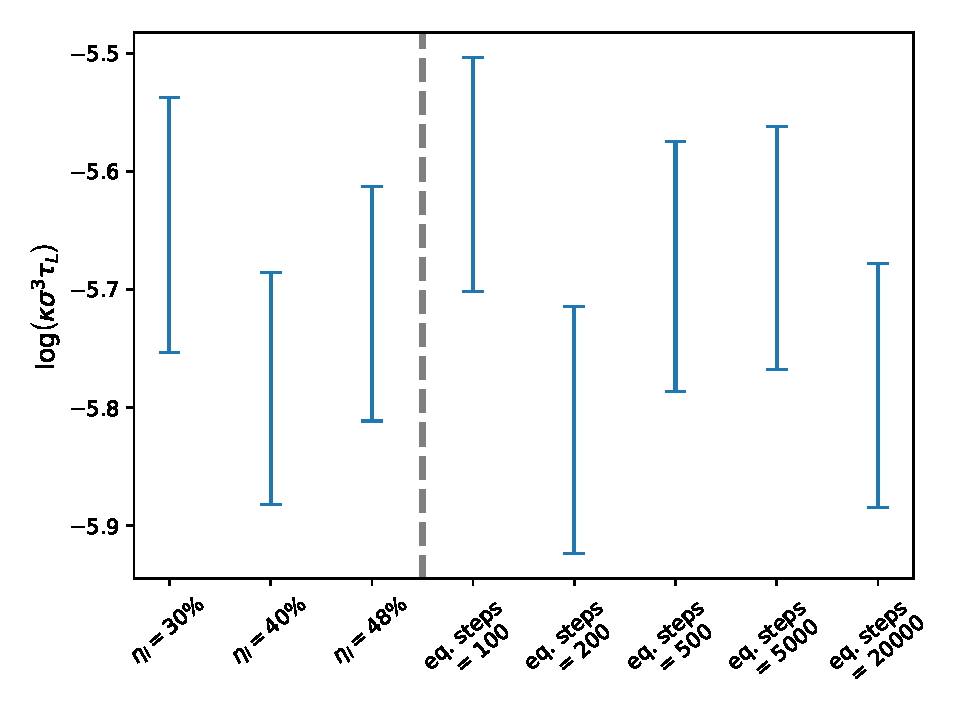
\includegraphics[width=1 \linewidth]{nucleation_rate_pre_comparison.pdf}
\caption[Nucleation rates of equilibration test measurements]{Nucleation rates for different start parameters }
\label{fig:comparison_nucleation_rates}
\end{figure}
}

\column{0.03 \linewidth}
\end{columns}
\end{frame}

\fi


\begin{frame}
\frametitle{Choice of Data Production Parameters}
\begin{itemize}
\item $\mathcal{O}(N)$ calculation effort
\begin{align*}
\label{eqn:system_size}
\Rightarrow  \frac{\delta T_{\text{CPU}}}{\delta t_{\text{Sim.}}} \propto N \propto V 
\end{align*}

\item Without initial induction time
\begin{align*}
\Rightarrow \langle \tau_{\text{Nucleation}} \rangle \propto \frac{1}{V}
\end{align*}

\item Time to nucleation
\begin{align*}
\Rightarrow  \langle T_{\text{CPU}} \rangle \propto  \frac{\delta T_{\text{CPU}}}{\delta t_{\text{Sim.}}}  \cdot \langle \tau_{\text{Nucleation}} \rangle \propto \text{const.}
\end{align*}
\vspace{0.1cm}

\quad $\Rightarrow$  Large system sizes possible
\end{itemize}
%\end{columns}
\end{frame}

\begin{frame}
\frametitle{Cluster Growth - Constant Attachment Rate}
\begin{columns}
\column{1 \linewidth}
\begin{itemize}
\item Constant attachment rate $\Rightarrow R \propto t$
\item Spherical growth $\Rightarrow V \propto R^3 \propto t^3  \quad \Rightarrow N(t) = c^3 (t-t_0)^3$
\end{itemize}
\end{columns}

\begin{columns}
\column{0.5 \linewidth}
\begin{figure}[h]
\centering
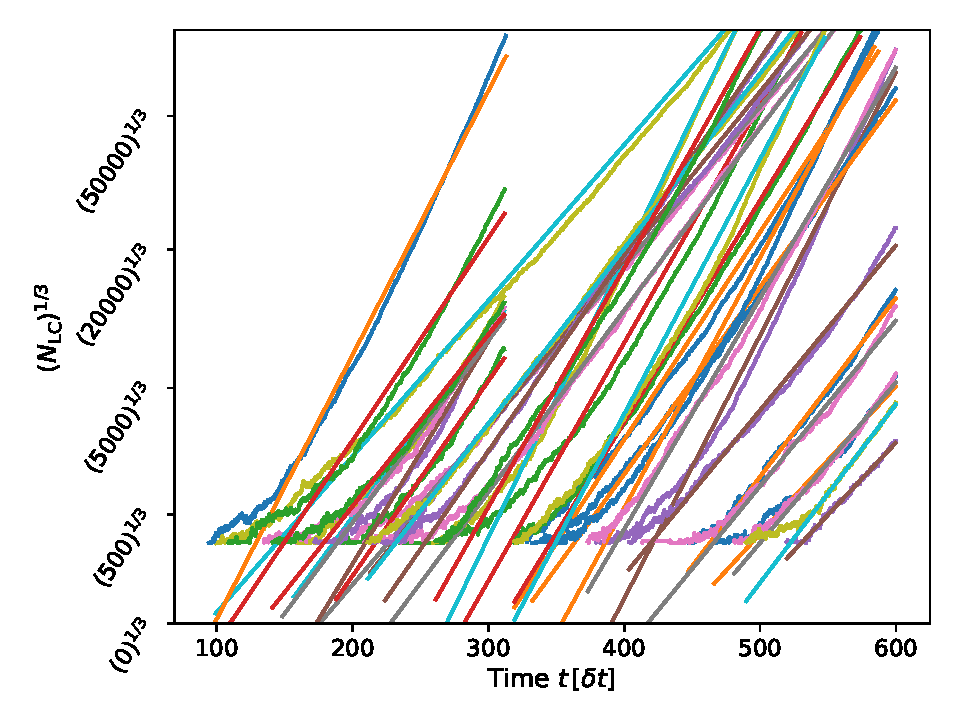
\includegraphics[width=1 \linewidth]{cluster_growth_example.pdf}
\caption[Largest cluster trajectories from production data with constant attachment rates]{Third root of the number of particles in the largest cluster}
\label{fig:cluster_growth_example}
\end{figure}
\column{0.5 \linewidth}

\begin{figure}[h]
\begin{center}
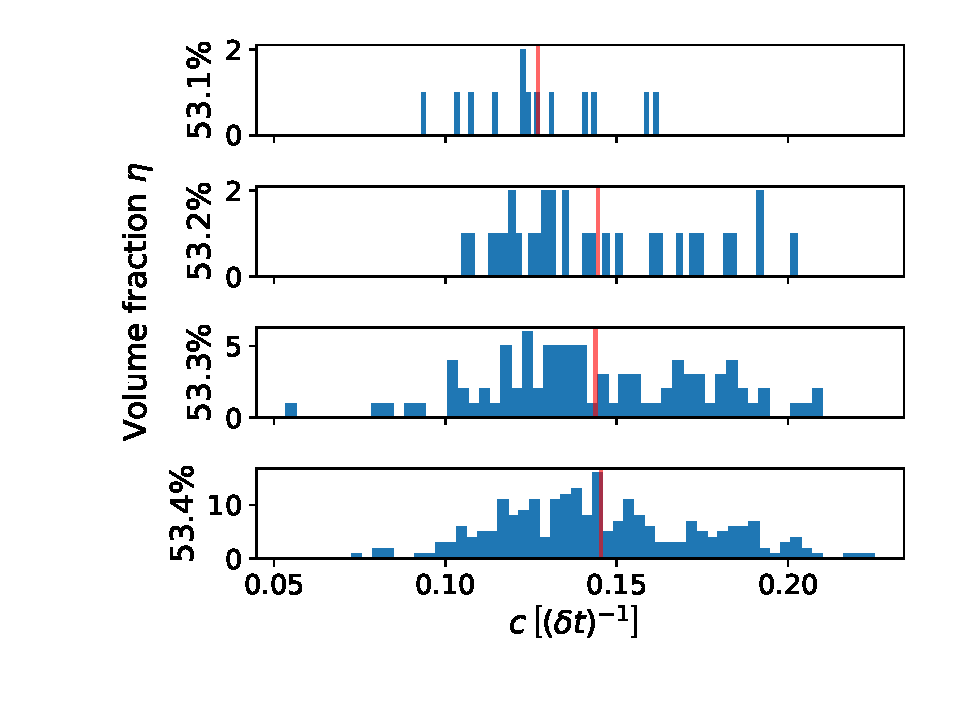
\includegraphics[width = 1 \textwidth]{const_growth_rate_histogram_comparison.pdf}
\caption[Constant attachment rate measurements from production data]{Comparison of growth rates in the constant attachment regime.}
\label{fig:constant_growth_rates}
\end{center}
\end{figure}
\end{columns}
\end{frame}


\begin{frame}
\frametitle{Nucleation Time Distribution}
Assume simulation geometry and $\kappa(t) =  \text{const.}$ \vspace{0.25cm}
\begin{itemize}
\item $N$ subvolumes of size $V_{box}$
\item $n(t$) nucleated boxes
%\item Assume $\kappa(t) =  \text{const.}$
\begin{align*}
\langle \Delta n \rangle &= (N - n(t))V_{\text{box}}\kappa \, \Delta t
\end{align*}
\item In the continuous limit of $N \rightarrow \infty $ with $V_{\text{box}}\kappa = k$
\begin{align*}
\Leftrightarrow  x_s &= \frac{n(t)}{N} = 1 - \exp\left( -t \, k\right)\\
\Leftrightarrow \dot{x_s} &= k \exp\left( -t \, k \right)
\end{align*}

%\item In the continous limit of $N \rightarrow \infty $ with $k = V_{\text{box}} \kappa $ 
%\begin{align*}
%\Leftrightarrow  x_s &= \frac{n(t)}{N} = 1 - \exp\left( -t \!\, k \right)\\
%\Leftrightarrow \dot{x_s} &= k \exp\left( -t  \!\, k \right) 
%\end{align*}

%\item In the continous limit of $N \rightarrow \infty $
%\begin{align*}
%\Leftrightarrow  x_s &= \frac{n(t)}{N} = 1 - \exp\left( -t V_{\text{box}}\kappa \right)\\
%\Leftrightarrow \dot{x_s} &= V_{\text{box}}\kappa \exp\left( -t V_{\text{box}}\kappa \right) 
%\end{align*}

$\Rightarrow$ Exponentially distributed nucleation times
\end{itemize}
\end{frame}


\iffalse

\begin{frame}
\frametitle{Nucleation Time Definition}
\begin{columns}
\column{0.5 \linewidth}
Possible "nucleation times": \vspace{0.25cm}\\

\begin{description}
\item[Horizon crossing:]{\hfill \\ \hspace{-1.5cm} No distinct largest cluster}

\item[Exponential extrapolation:]{\hfill \\ \hspace{-1.5cm} Fit to initial growth below 10}

\item[Constant extrapolation:]{\hfill \\ \hspace{-1.5cm} Later growth extrapolated to 0}
\end{description}


\column{0.5 \linewidth}
\begin{figure}[!h]
\centering
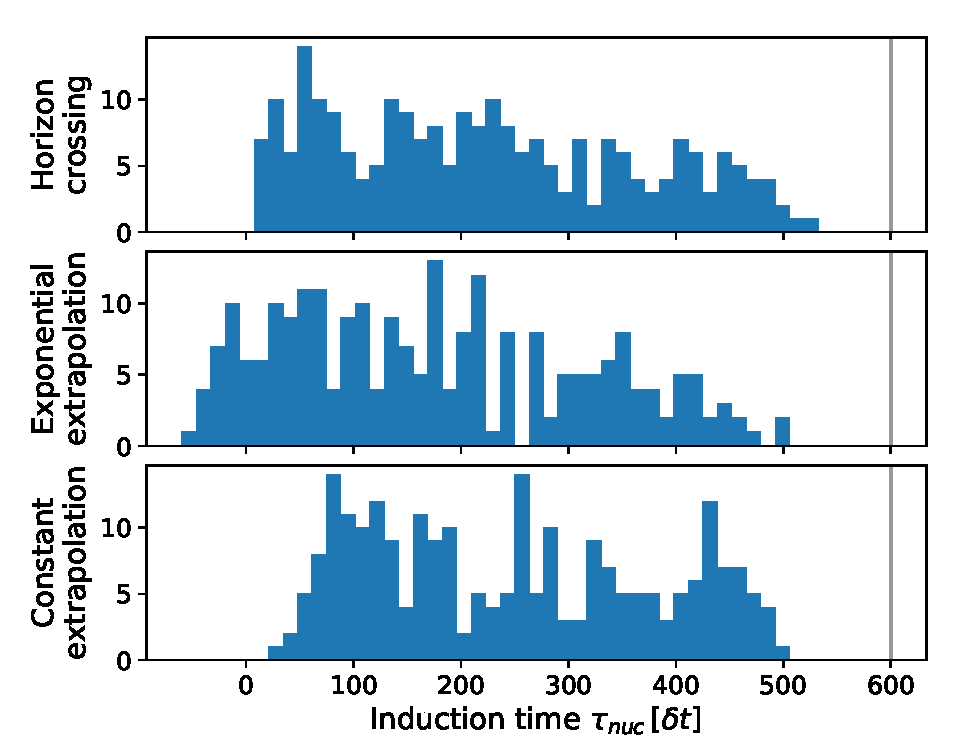
\includegraphics[width=1.0 \linewidth]{varying_induction_time.pdf}
\caption[Comparison of different definitions for the induction time]{Induction time distribution obtained by different definitions.}
\label{fig:induction_distributions}
\end{figure}

\end{columns}
\end{frame}

\fi

%\begin{frame}
%\frametitle{Nucleation Rate Estimator I -\\ \hfill Maximum Log-Likelihood Estimator}
%\begin{itemize}
%\item Probability Density Function of censored exponential distribution
%\begin{align*}
%p(t) = 
%\begin{cases}
%\kappa \exp(-\kappa t) & t < T\\
%\exp(-\kappa T) & t \geq T\\ 
%\end{cases}
%\end{align*}

%\item Likelihood of measurement
%\begin{equation*}
%\mathcal{L}(\kappa)  =  \binom{N}{m} \;  \kappa^n \; \exp(- \kappa \sum_{i=1}^n t_i) \;  \exp(-\kappa T)^{m} \quad %\right| \left.\frac{\partial \log ( ... )}{\partial \kappa} \right|_{\kappa=\hat{\kappa}}
%\end{equation*}

%\item Necessary condition of maximum likelihood
%\begin{equation*}
%\hat{\kappa}^{-1} = \frac{1}{n} \left(  \sum_{i=1}^n t_i + m T \right)
%\end{equation*}
%\end{itemize}
%\end{frame}




\begin{frame}
\frametitle{Nucleation Rate Estimator I -\\ \hfill Maximum Log-Likelihood Estimator}
\begin{itemize}
\item Probability Density Function of censored exponential distribution
\begin{align*}
p(t) = 
\begin{cases}
k \exp(-t \, k) & t < T\\
\exp(- T \, k) & t \geq T\\ 
\end{cases}
\end{align*}

\item Likelihood of measurement
\begin{equation*}
\mathcal{L}(k)  =  \binom{N}{m} \;  k^{n} \; \exp\left(- k \sum_{i=1}^n t_i \right) \;  \exp\left(-T \, k \right)^{m} \quad %\right| \left.\frac{\partial \log ( ... )}{\partial \kappa} \right|_{\kappa=\hat{\kappa}}
\end{equation*}

\item Necessary condition of maximum likelihood
\begin{equation*}
\hat{k}^{-1} = \frac{1}{n} \left(  \sum_{i=1}^n t_i + m T \right)
\end{equation*}
\end{itemize}
\end{frame}



\begin{frame}
\frametitle{Nucleation Rate Estimator II -\\ \hfill Monte Carlo Uncertainty}
\begin{columns}
\column{0.5 \linewidth}
\begin{enumerate}
\item Exponentially distributed random samples with $k = \hat{k}$
\item Censoring at T
\item Calculate $\hat{k}_{MC}$
\item<2> $\sigma_{\hat{k}}$ estimated by $\sigma_{\hat{k}_{MC}}$
\end{enumerate}

\column{0.47 \linewidth}

\only<1>{\begin{figure}[ht]
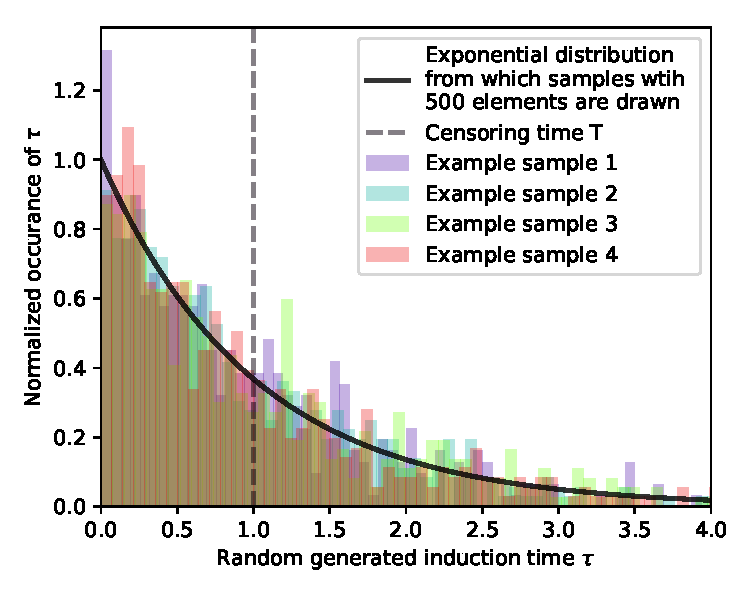
\includegraphics[width = 1.0 \textwidth]{mc_random_sample.pdf}
\end{figure}}

\only<2>{\begin{figure}[ht]
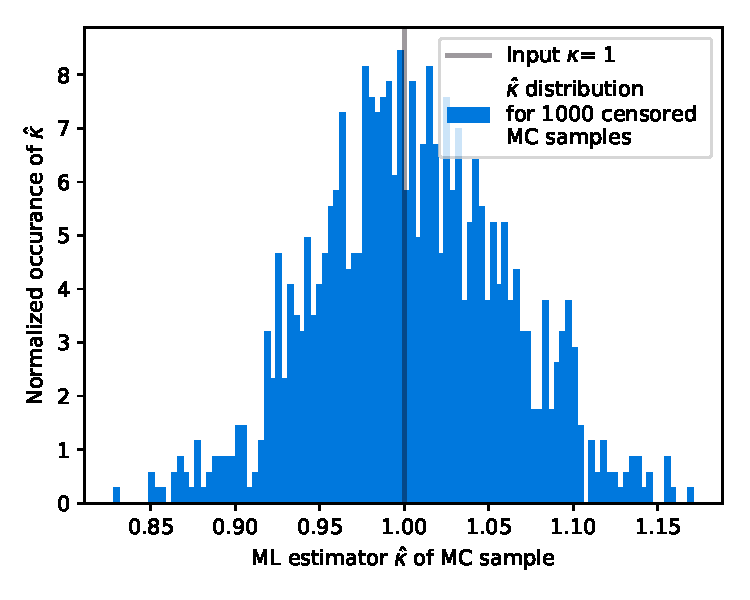
\includegraphics[width = 1.0 \textwidth]{k_estimator_distribution.pdf}
\end{figure}}

\column{0.03 \linewidth}
\end{columns}
\end{frame}






%\begin{frame}
%\frametitle{Nucleation Rate Estimator II -\\ \hfill Monte Carlo Uncertainty}
%\begin{columns}
%\column{0.5 \linewidth}
%\begin{enumerate}
%\item Exponentially distributed random samples with $\kappa = \hat{\kappa}$
%\item Censoring at T
%\item Calculate $\hat{\kappa}_{MC}$
%\item<2> $\sigma_{\hat{\kappa}}$ estimated by $\sigma_{\hat{\kappa}_{MC}}$
%\end{enumerate}

%\column{0.47 \linewidth}

%\only<1>{\begin{figure}[ht]
%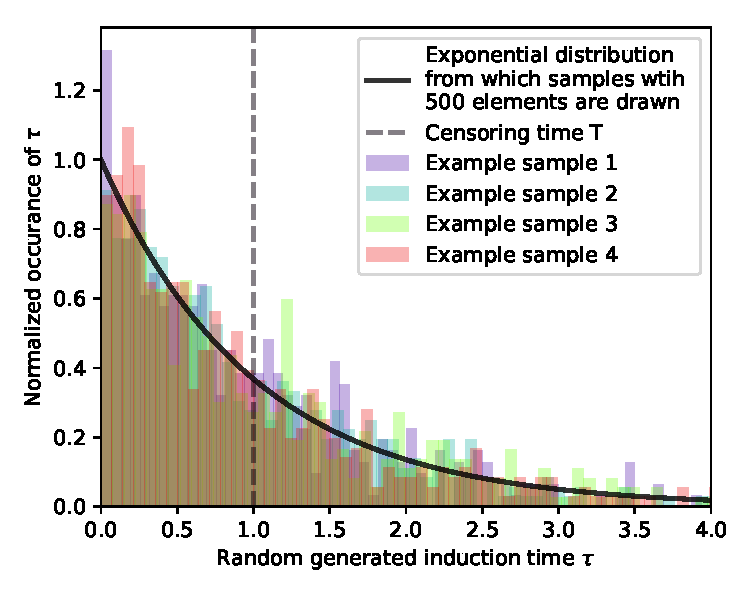
\includegraphics[width = 1.0 \textwidth]{mc_random_sample.pdf}
%\end{figure}}

%\only<2>{\begin{figure}[ht]
%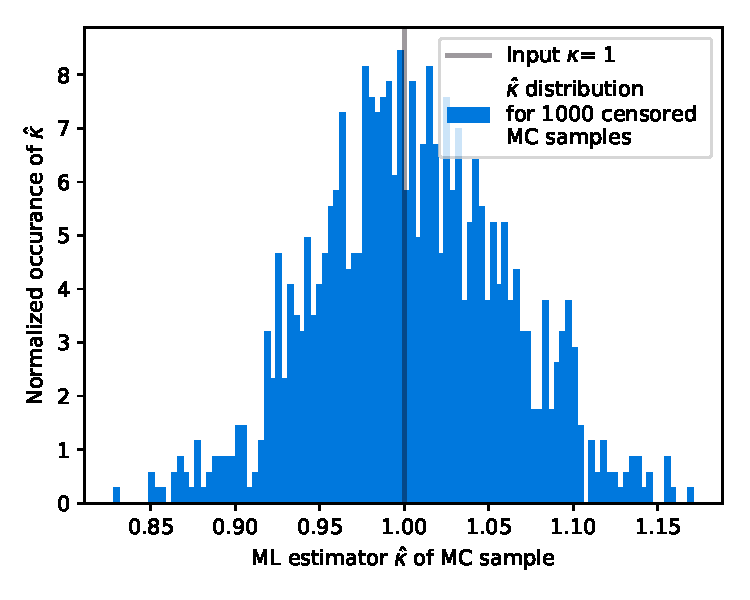
\includegraphics[width = 1.0 \textwidth]{k_estimator_distribution.pdf}
%\end{figure}}

%\column{0.03 \linewidth}
%\end{columns}
%\end{frame}

\begin{frame}
\frametitle{Nucleation Rate Comparison}
\begin{columns}
\column{0.73 \linewidth}
\begin{figure}[h]
\centering
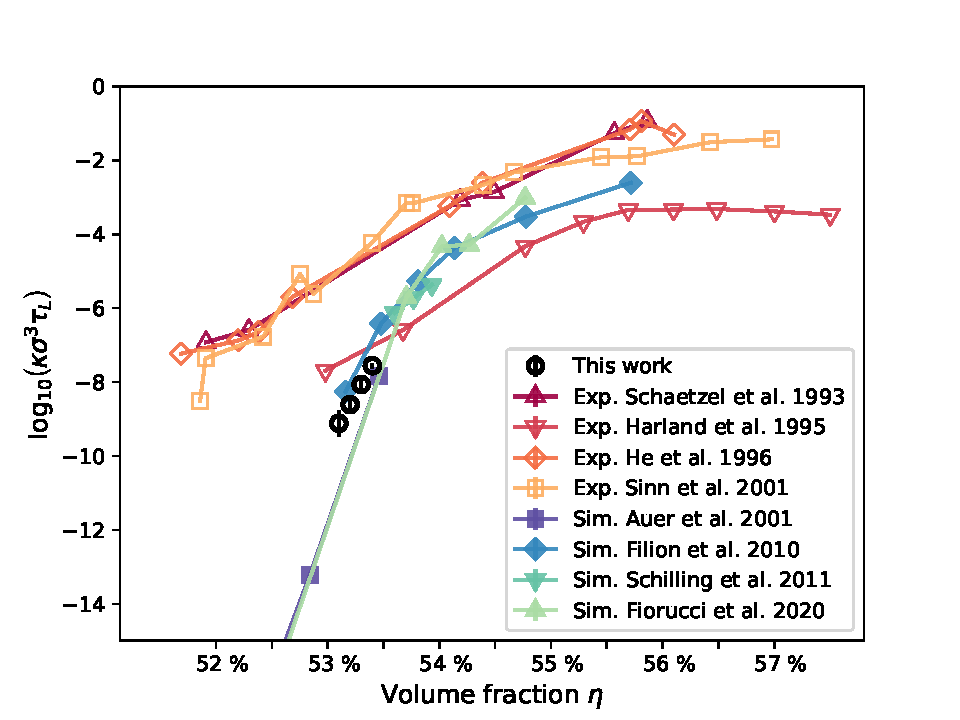
\includegraphics[width=1 \linewidth]{nucleation_comparison_v2.pdf}
\caption[]{Experimental and theoretical nucleation rates from the literature\cite{Harland1997,He1996,schaetzel1993,Sinn2001,Auer2001,Filion2010a,Fiorucci2020a,Schilling2011}}
\end{figure}

\column{0.27 \linewidth}
Simulations and experiments:\\

\begin{itemize}
\item Different rates
\item Different slopes
\end{itemize}
\end{columns}
\end{frame}

\begin{frame}
\frametitle{Comparison to Real World Experiments}
%\begin{itemize}
%\item Solid fraction of infinite volume $ N(t)=\kappa V \int_0^{t} c^3 (t - t')^3 d t'$
%\item Avrami model for 
%\item
\begin{table}
\begin{center}
\begin{tabular}{c||c}
Simulation & Experiment\raisebox{-0.2cm}{ \makebox[0.0cm]{}}  \\ \hline \hline
Microscopic disjunct subvolumes & Macroscopic volume  \raisebox{-0.2cm}{ \makebox[0.0cm]{}} \raisebox{0.4cm}{ \makebox[0.0cm]{}} \\ \hline
%One cluster per box & Many clusters per box\\ \hline
$\tau_{cryst.} \ll \tau_{nuc.}$ & $\tau_{cryst.} \ll \!\!\!\!\!\!/ \; \tau_{nuc.}$  \raisebox{-0.2cm}{ \makebox[0.0cm]{}} \raisebox{0.35cm}{ \makebox[0.0cm]{}}\\ \hline
$x_s \approx \frac{n(t)}{m} = 1 - \exp (- \kappa t)$ & $x_s(t) = t^4 \frac{\kappa c^3}{4 \rho_{\text{melt}}} $, $x_s \ll 1$ \raisebox{-0.2cm}{ \makebox[0.0cm]{}} \raisebox{0.4cm}{ \makebox[0.0cm]{}}
\end{tabular}
\end{center}
\end{table}
\vspace{0.2cm}
\begin{itemize}
\item $\kappa$ and c are measured
%\item Steep increase when $x_s(t) \ll \!\!\!\!\!\!/ \; 1$  at  $ t^* $
\item Assume $x_s(t^*) \stackrel{!}{=} 1/8$ \quad  $ \Rightarrow t^* = \sqrt[4]{\frac{\rho_{\text{melt}}}{2 \kappa c^3 }} $ 
\end{itemize}
\end{frame}

\begin{frame}
\frametitle{Modified Nucleation Rate Comparison}

\begin{columns}
\column{0.73 \linewidth}
\begin{figure}[h]
\centering
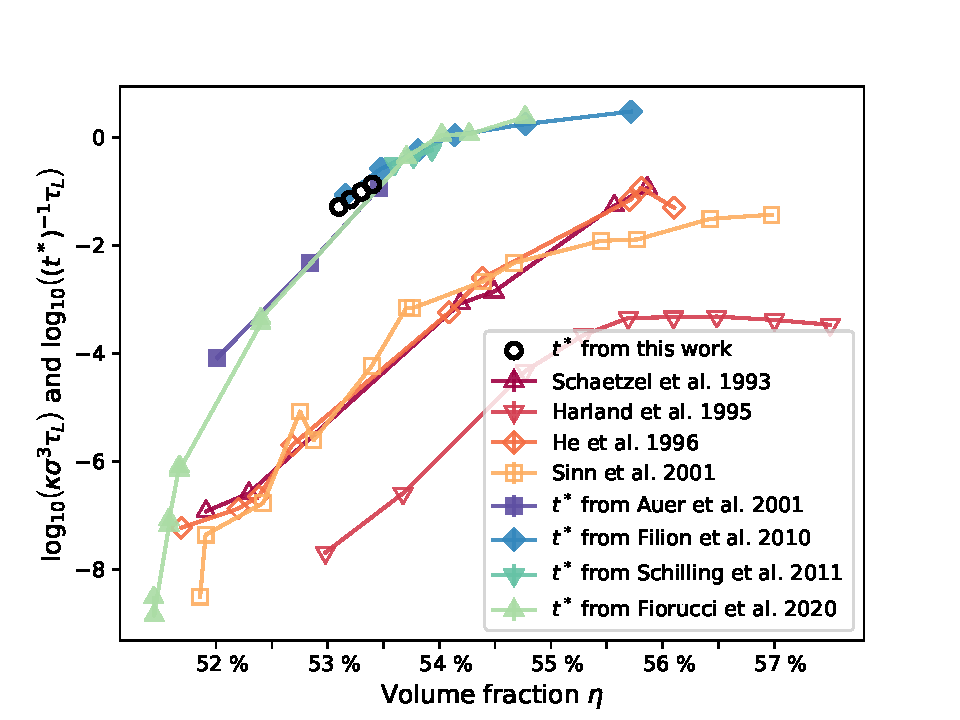
\includegraphics[width=1.0 \linewidth]{mod_nucleation_comparison_v2.pdf}
\caption[Nucleation rate comparison under assumption of early filled boxes]{Experimental nucleation rates\cite{Harland1997,He1996,schaetzel1993,Sinn2001,Auer2001} alongside with $(t^*)^{-1}$ calculated from simulation studies\cite{Filion2010a,Fiorucci2020a,Schilling2011}}
\label{fig:nucleation_rate_comparison_modified}
\end{figure}


\column{0.27 \linewidth}
Simulations and experiments:\\

\begin{itemize}
\item Different rates
\item Similar slopes
\end{itemize}
\end{columns}






\end{frame}

\begin{frame}
\frametitle{Memory Kernel I - Largest Cluster Trajectories}
Last but not least,\\
\begin{center}
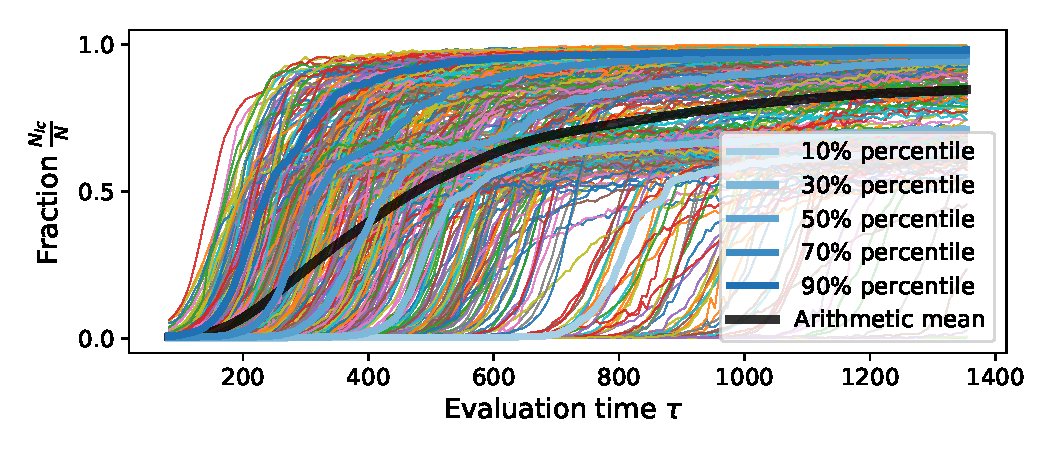
\includegraphics[width=0.7 \linewidth]{largest_cluster_trajectories.pdf}
\end{center}

\begin{columns}
\column{0.05 \linewidth}
\column{0.45 \linewidth}
\begin{itemize}
\item N = 16384 particles
\item $\eta = 54.0 \%$
\end{itemize}
\column{0.5 \linewidth}
\begin{itemize}
\item $\tau_{ind.} \approx 400 \delta t$
\item $\tau_{cry.} \approx 150 \delta t$
\end{itemize}
\end{columns}




\end{frame}

\begin{frame}
\frametitle{Memory Kernel II -Shape Analysis}
\begin{columns}
\column{ 0.4 \linewidth}
\only<1>{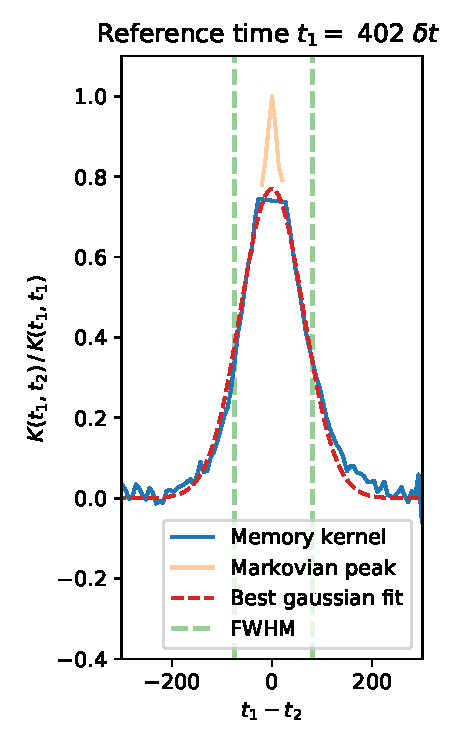
\includegraphics[width=1.0 \linewidth]{example_memory_kernel.pdf}}
\only<2>{
\begin{itemize}
%\item Memory described by Gaussian
\item Constant width $\sim \tau_{cry.}$
%\item Widht $\sim \tau_{cry.}$\\ 
%$\Rightarrow$ Visible memory related to box size
\item Variable amplitude
%\item $\tau_{cry.}$ not related to dynamics $\Rightarrow$ 
\end{itemize}}
\column{0.6 \linewidth}
\only<1>{
%\begin{center}
%\centering
%\movie[label=mov1, width=6cm, height=5.95cm, showcontrols]{Memory kernel shape}{../../python/%kernel_width/movie.mp4}
%\end{center}
Shape analysis: \vspace{0.25cm}\\
\begin{itemize}
\item Exclude Markovian contribution
\item FWHM of crest as first estimate
\item Best Gaussian fit as second estimate
\end{itemize}

}
\only<2>{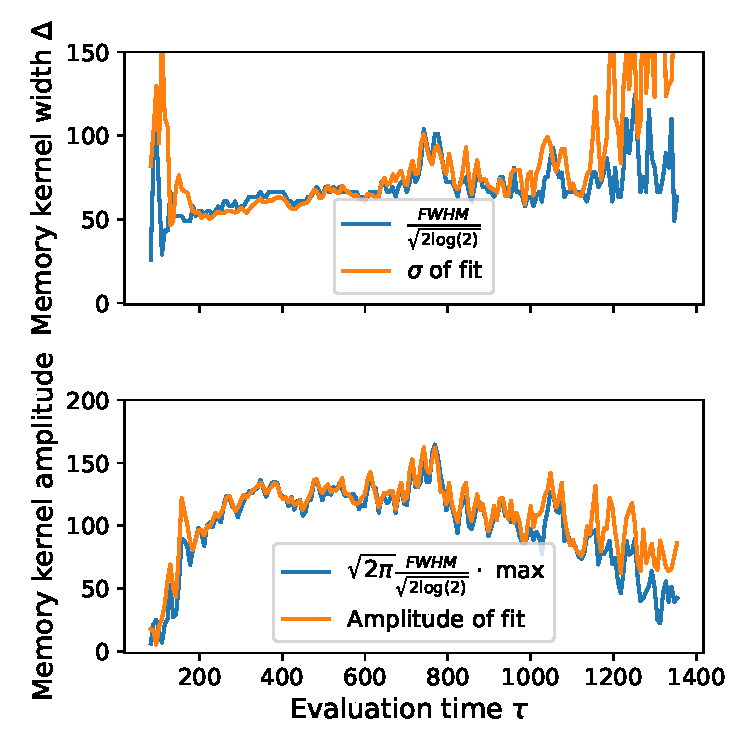
\includegraphics[width=1 \linewidth]{memory_kernel_shape.pdf}}

\end{columns}
$\Rightarrow$ Possibly only memory depending on the arbitrary transition width is observed.
\end{frame}

%\begin{frame}
%\frametitle{Memory Kernel III - Shape Analysis}
%\end{frame}

\begin{frame}
\frametitle{Conclusion - Summary}
\begin{itemize}
%\item Importance of phase transitions
%\item EDMD simulation code
\item Constant attachment rate
%\item Induction time measurement
\item Estimate of nucleation rate density + statistical uncertainty\\
$\Rightarrow$ Confirming the difference
%\item Nucleation rate density measurement
\item System geometries in simulation and experiment\\
$\Rightarrow$ Possible accordance \vspace{0.25cm}
\item Memory kernel shape analysis\\
$\Rightarrow$ Future research in other observables
\end{itemize}
\end{frame}

\begin{frame}
\frametitle{\makebox[0.1cm]{}}
\begin{center}
\makebox{\huge Thank you for your attention}
\end{center}
\begin{columns}
\column{0.5 \linewidth}
\begin{figure}[h]
\centering
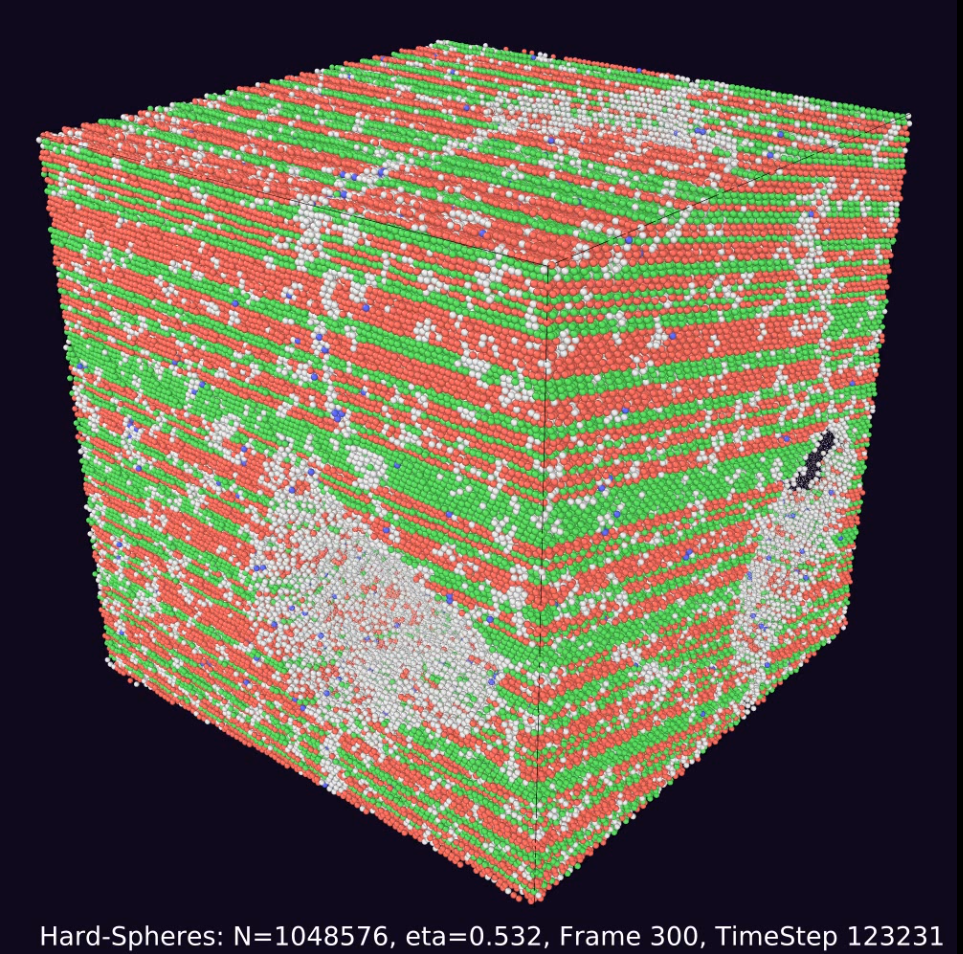
\includegraphics[width=0.8 \linewidth]{animation_poster_532_cc.png}
%\caption[]{}
\end{figure}


\column{0.5 \linewidth}
\begin{figure}[h]
\centering
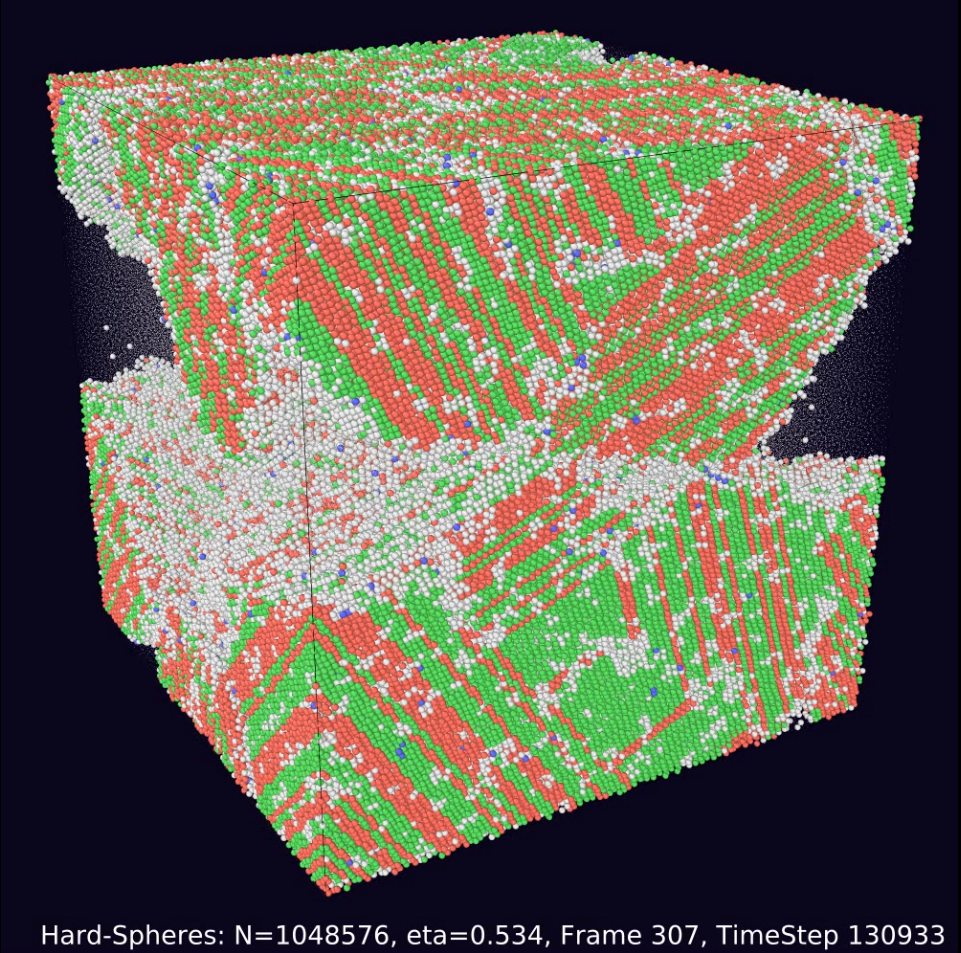
\includegraphics[width=0.8 \linewidth]{animation_poster_534_cc.png}
%\caption[]{}
\end{figure}


\end{columns}
\end{frame}


%\begin{frame}
%\begin{figure}[h!]
%\centering
%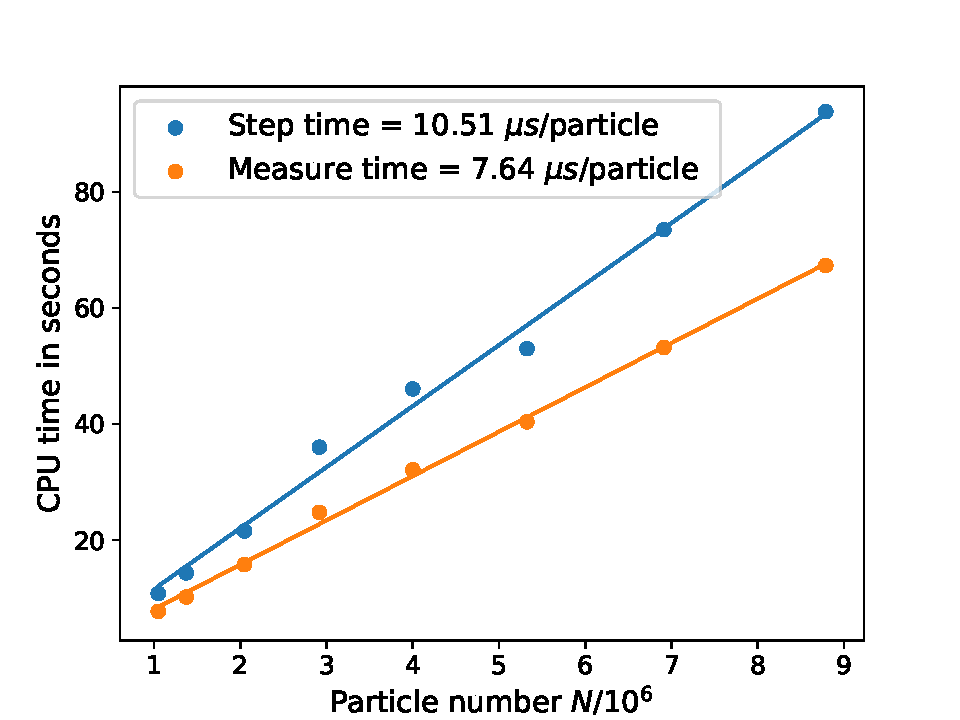
\includegraphics[width=0.5 \linewidth]{Calculation_times_measurement.pdf}
%\caption[Calculation time estimate of the simulation]{Overview of CPU time required for calculating a simulation step, consisting of an event for each particle, as well as a measurement of relevant quantities of the system. As assumed for a simulation algorithm with a theoretical $\mathcal{O}(N)$ calculation effort, the data points can be well described by a line. As the CPU time is clearly related to the further workload of the CPU during the calculation it is also expected to find fluctuations if the other workload of the machine is not strictly controlled.}
%\label{fig:calc_time}
%\end{figure}
%\end{frame}
\begin{frame}[allowframebreaks]{Bibliography}
	\printbibliography{}
\end{frame}
\end{document}

